\section{UI Designs}
In diesem Kapitel sollen die verschiedenen Versionen unseres UI Designs geführt werden.

\subsection{Recherche UI Designs}

Zuerst haben wir uns mehrere UI Designs von verschiedenen Quellen angeschaut, um einen besseren Überblick über die
Designmöglichkeiten zu bekommen.
\\

\newcolumntype{C}[1]{>{\centering\let\newline\\\arraybackslash\hspace{0pt}}m{#1}}
\newcolumntype{L}[1]{>{\raggedright\let\newline\\\arraybackslash\hspace{0pt}}m{#1}}


\begin{tabular}{C{6cm}  L{7cm}}
    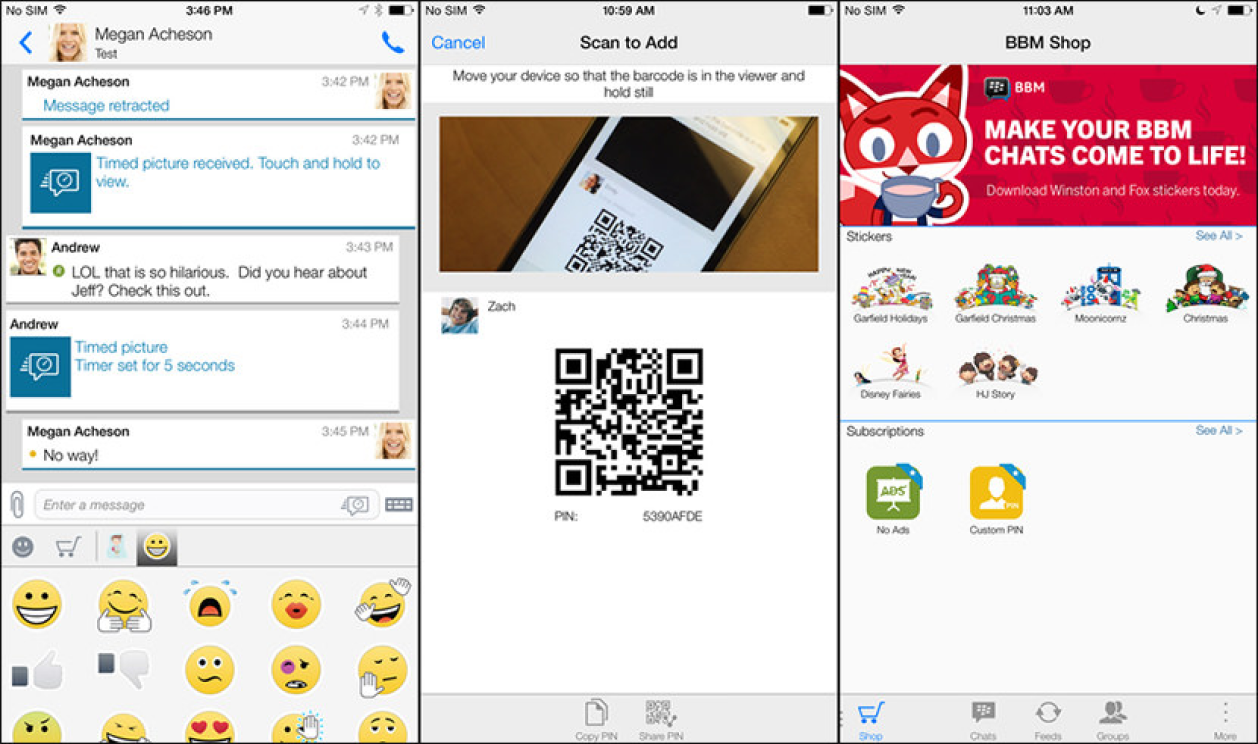
\includegraphics[width=\linewidth]{bilder/research pic/blackberry-messenger-live-free.png}
                                                                                        & \textbf{Blackberry Messenger Live}\newline
    Zuerst haben wir uns umgeschaut und nach Chatfenstern gesucht. Hier haben wir uns die Austauschung von Sprechblasen angeschaut
    und deren Ausrichtung.                                                                                                           \\
    Bildquelle:\cite{blackberry} \newline                                                                                            \\
    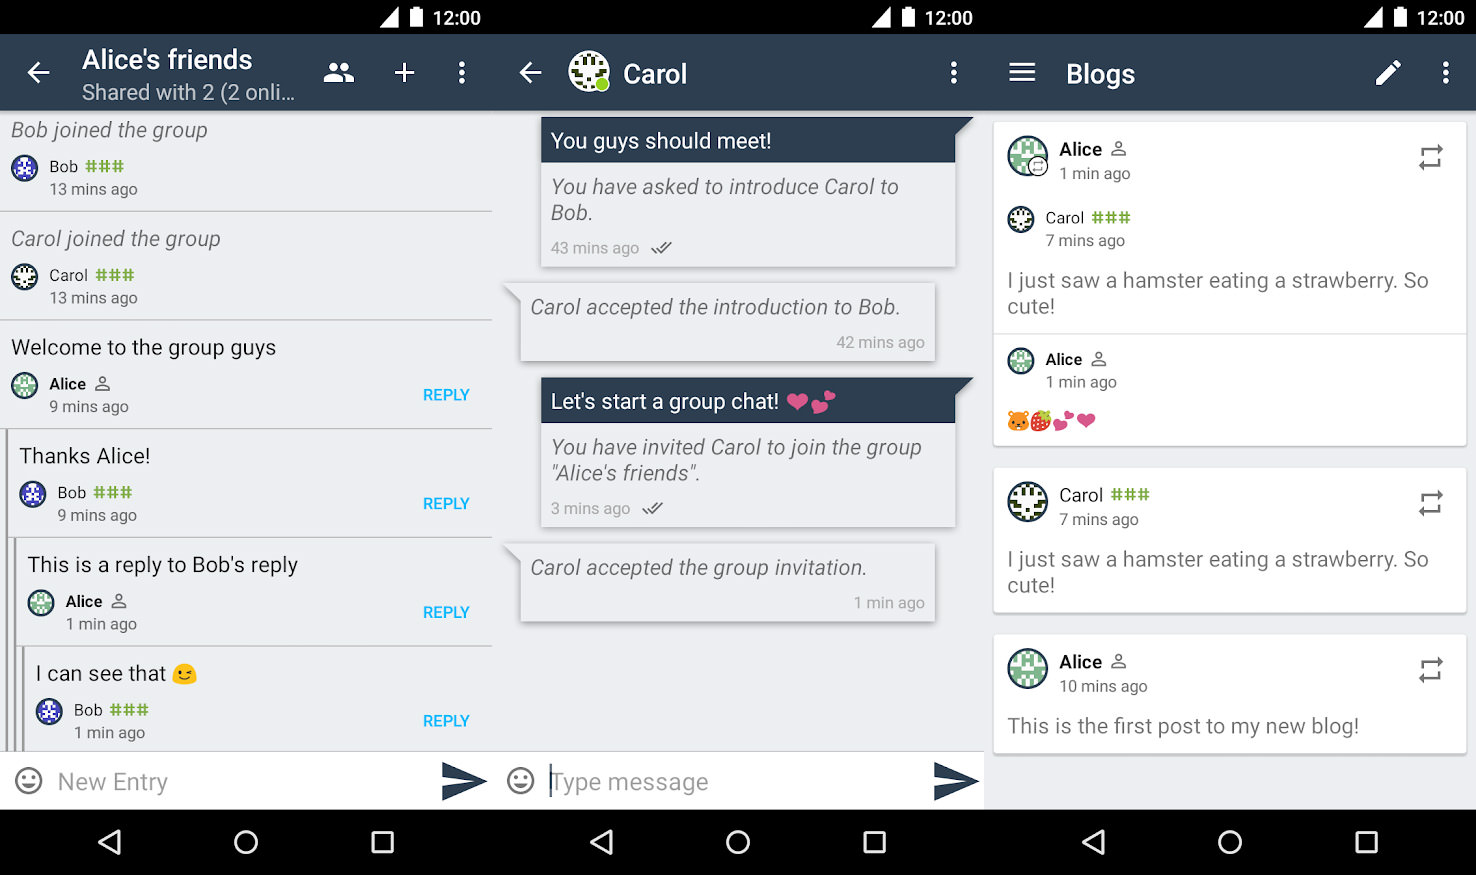
\includegraphics[width=\linewidth]{bilder/research pic/briar.jpg}
                                                                                        & \textbf{Briar} \newline
    In diesem Beispiel haben wir uns wieder das Chatfenster und die verschiedenen Symbole angeschaut.
    Wie den Editierbutton oder den Hinzufügebutton.                                                                                  \\
    Bildquelle:\cite{briar} \newline                                                                                                 \\
    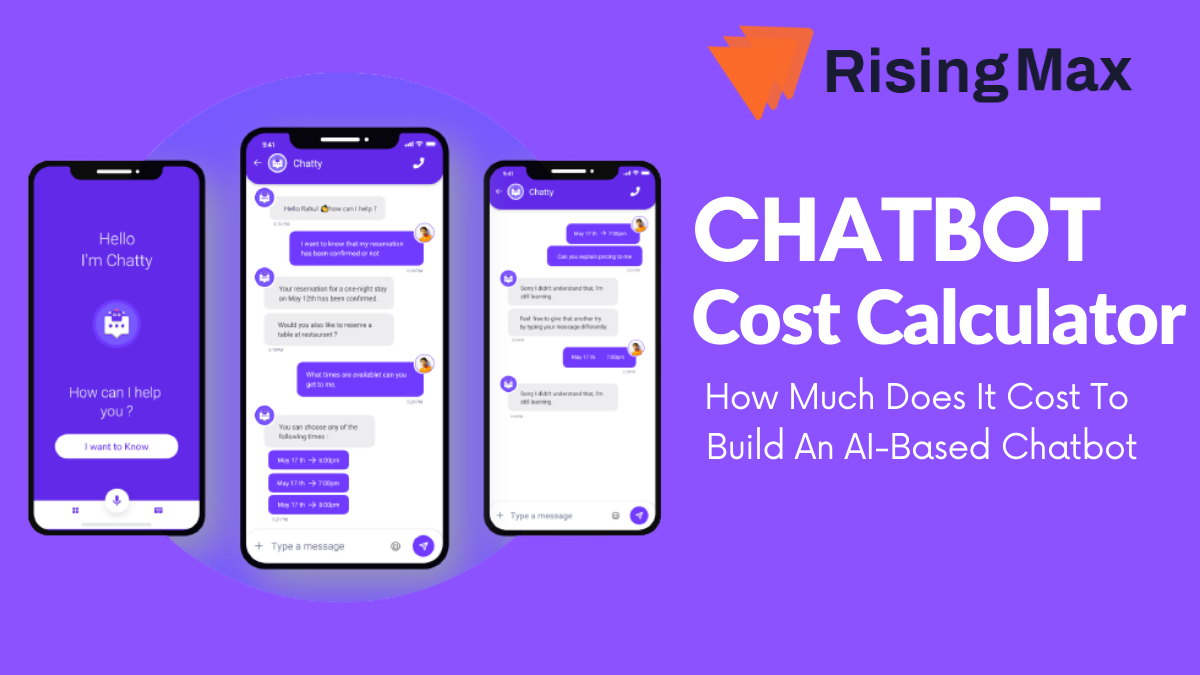
\includegraphics[width=\linewidth]{bilder/research pic/chatbot-cost-calculator.png} & \textbf{CHATBOT Cost Calculator} \newline
    Hier haben wir uns ein ChatBot-Fenster angeschaut und dabei die Icons und die
    verschiedenen Elemente angeschaut, wie den Balken an der Oberseite oder den Sendebutton.                                         \\
    Bildquelle:\cite{chatbotcostcalc} \newline
\end{tabular}

\begin{tabular}{C{6cm}  L{7cm}}
    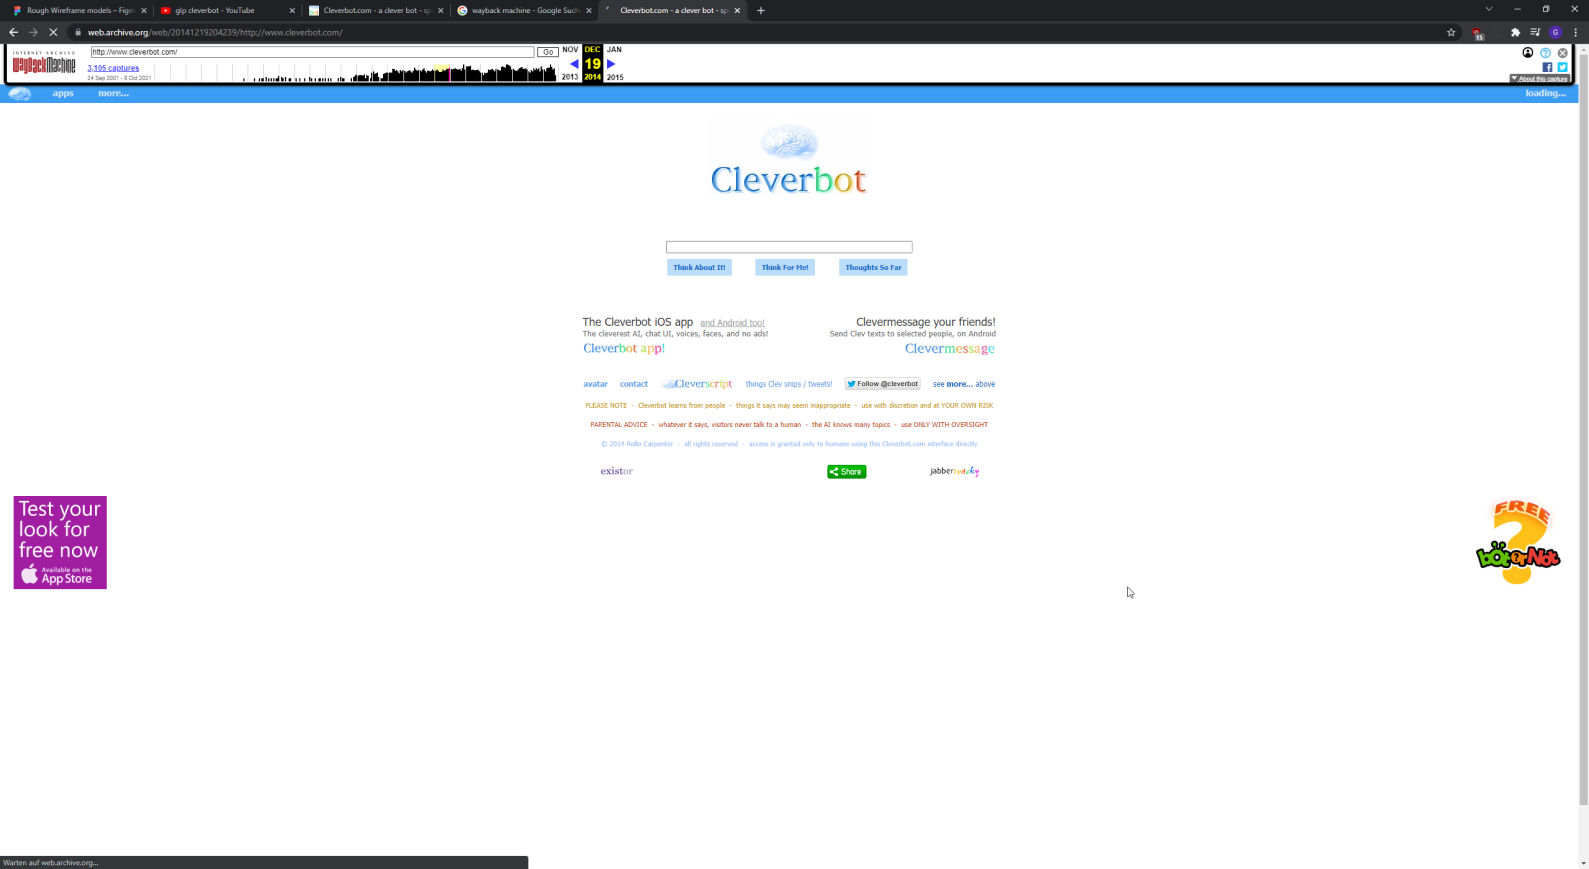
\includegraphics[width=\linewidth]{bilder/research pic/cleverbot.png}                 & \textbf{Cleverbot} \newline
    Diesen Bot haben wir uns genauer angeschaut, weil dieser auch uns bekannt war.                                      \\
    Bildquelle:\cite{cleverbot} \newline
    \\
    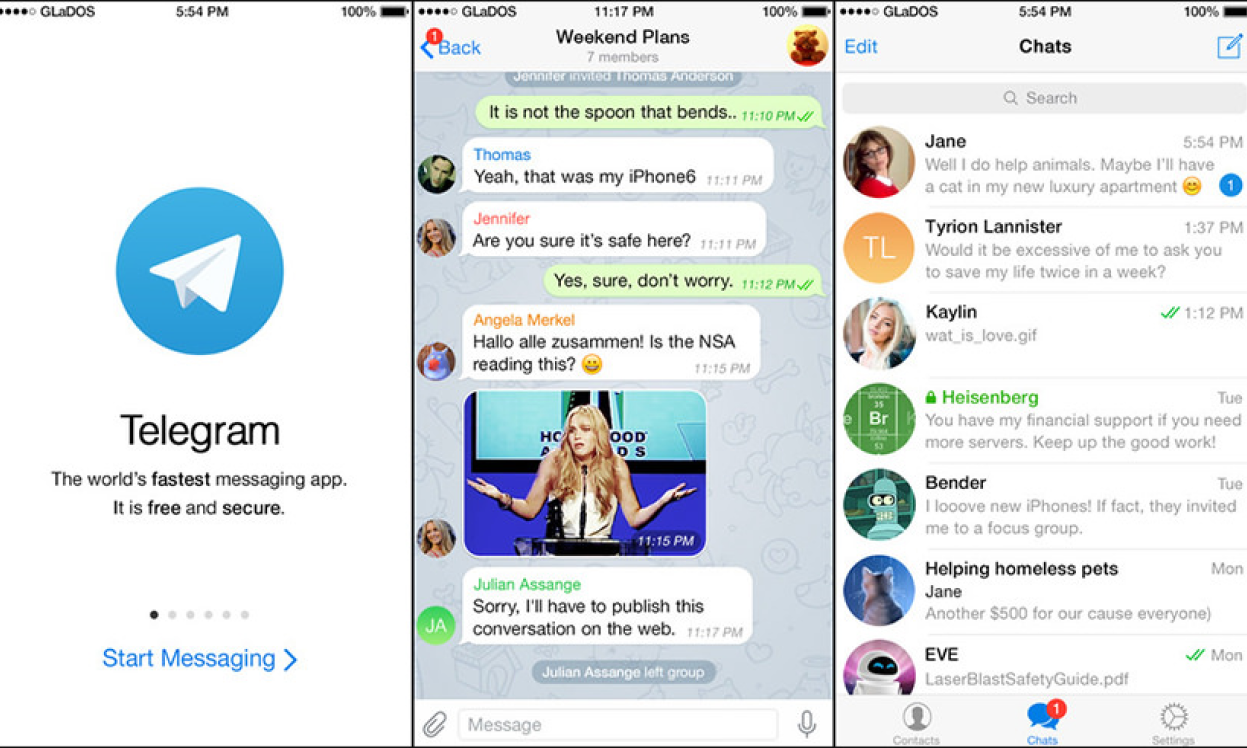
\includegraphics[width=\linewidth]{bilder/research pic/Telegram pic.png}              & \textbf{Telegram} \newline
    Telegram haben wir uns wiederum das Chatfenster und die Icons angeschaut.                                          \\
    Bildquelle:\cite{telegrambild} \newline
    \\
    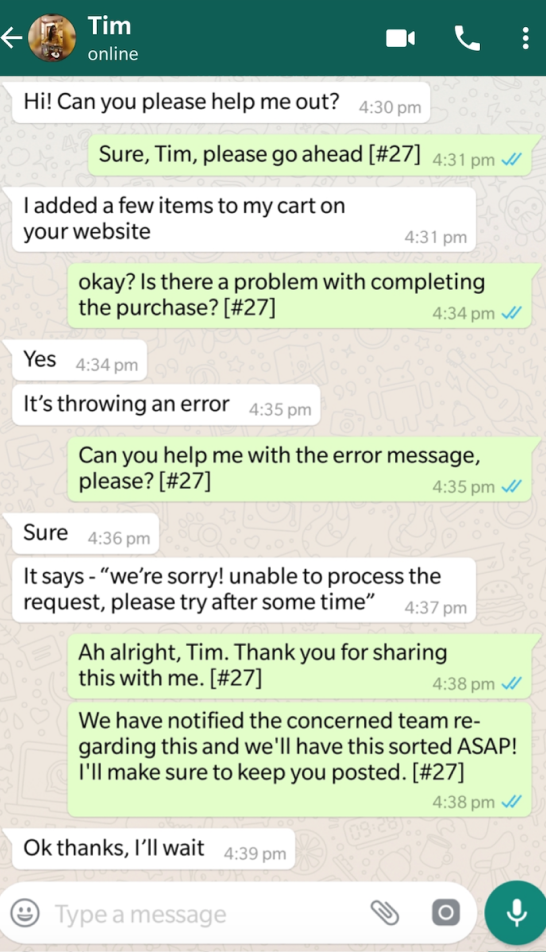
\includegraphics[width=\linewidth, height=12cm]{bilder/research pic/Tim Whatsapp.png} & \textbf{WhatsApp} \newline
    Hier haben wir uns mehr auf die Ausrichtungen des Chatfensters angeschaut und wie die Sprechblasen
    ausgerichtet sind. Fast jeder benutzt WhatsApp, deswegen haben wir uns die Struktur angeschaut,
    weil diese vielen Benutzern bekannt ist.                                                                              \\
    Bildquelle:\cite{timwhatsApp} \newline
\end{tabular}

\subsection{Erfahrungen zu der Recherche von unseren UI Designs}
In Recherche von den UI Designs haben die einzelnen Komponenten wie der Aufbau eines Chats und 
die Anordnung eine große Rolle gespielt. Die Erfahrungen, die man aus den einzelnen Elementen gesammelt hat,
sind:
\\

\noindent Die Chatfenster sind immer gleich aufgebaut. 
Sie haben alle eine große Fläche, wo die Chats angezeigt werden. 
Außerdem haben alle Chat Designs ein Textfeld, wo man seine Fragen und Anliegen schreiben kann. 
Jeder User besitzt ein Profilbild. Sogar der ChatBot besitzt ein Profilbild. 
Das Chatfeld vom ChatBot Calculator hat ein gutes Design, wo das Profilbild neben dem Chatfeld zu sehen ist.
Demnach ist nachvollziehbar, wer was geschrieben hat. 
Neben dem Textfeld, wo man seine Anliegen eingeben kann, steht immer der Sendebutton.
Die Benutzer sind also mehr auf ein UI Design eingestellt, welches ihnen immer vorgelegt wird.
Darum wird das questMe Chatfenster auch ein UI Design erhalten, welches sich von der 
Basisstruktur der anderen Chats im Alltag nicht unterscheidet.



